\documentclass{anstrans}
%%%%%%%%%%%%%%%%%%%%%%%%%%%%%%%%%%%
\title{Multiphysics Techniques for Neutron Diffusion Using Improved Quasi-Static Method}
\author{Zachary M.~Prince, Jean C. Ragusa}

\institute{
Department of Nuclear Engineering, Texas A\&M University, College Station, TX
}

\email{zachmprince@tamu.edu \and jean.ragusa@tamu.edu}

%%%% packages and definitions (optional)
\usepackage{color} % allows inclusion of graphics
\usepackage{graphicx} % allows inclusion of graphics
\usepackage{booktabs} % nice rules (thick lines) for tables
\usepackage{microtype} % improves typography for PDF
\usepackage{subcaption}

\newcommand{\SN}{S$_N$}
\renewcommand{\vec}[1]{\bm{#1}} %vector is bold italic
\newcommand{\vd}{\bm{\cdot}} % slightly bold vector dot
\newcommand{\ud}{\mathop{}\!\mathrm{d}} % upright derivative symbol
%  new definitions
\newcommand{\bs}[1]{\mathbf{#1}}
\renewcommand{\div}{\bs{\nabla}\! \cdot \!}
\newcommand{\grad}{\bs{\nabla}}
% extra space
\newcommand{\qq}{\quad\quad}
% common reference commands
\newcommand{\eqt}[1]{Eq.~(\ref{#1})}                     % equation
\newcommand{\fig}[1]{Fig.~\ref{#1}}                      % figure
\newcommand{\tbl}[1]{Table~\ref{#1}}                     % table
\newcommand{\sct}[1]{Section~\ref{#1}}                   % section
\newcommand{\app}[1]{Appendix~\ref{#1}}                   % appendix

\newcommand{\keff}{k_\textit{eff}}

\newcommand{\be}{\begin{equation}}
\newcommand{\ee}{\end{equation}}
\newcommand{\vn}{\vec{n}}
\newcommand{\vel}{\vec{\mathrm{v}}}
\newcommand{\adj}{\Phi^\dagger_0}
\newcommand{\tcr}[1]{\textcolor{red}{#1}}
\newcommand{\norm}[1]{\left\lVert#1\right\rVert_{L^2}}


\begin{document}
%%%%%%%%%%%%%%%%%%%%%%%%%%%%%%%%%%%%%%%%%%%%%%%%%%%%%%%%%%%%%%%%%%%%%%%%%%%%%%%%
\section{Introduction}
The purpose of this summary is to introduce several techniques in dealing with temperature feedback for quasi-static neutron diffusion calculations.  Temperature is tightly coupled with neutron flux when simulating a nuclear reactor, thus it is a very important quantity to evaluate accurately and efficiently.  The improved quasi-static method (IQS) is an effective technique in simulating flux in reactors and the effect of multiphysics with IQS is worth exploring..

IQS is a transient spatial kinetics method that involves factorizing neutron flux into a space- and time-dependent component (shape) and a time-dependent component (amplitude) \cite{Ott_1966,Dulla2008}. The technique relies on the shape being less rapidly varying in time compared to the flux, hence requiring fewer shape computations or updates. IQS has mostly been applied to neutron kinetics, without thermal-hydraulic feedback. This summary discusses the application of temperature feedback with IQS and analyzes performance with benchmark problems

%%%%%%%%%%%%%%%%%%%%%%%%%%%%%%%%%%%%%%%%%%%%%%%%%%%%%%%%%%%%%%%%%%%%%%%%%%%%%%%%
\section{Theory}
In this Section, we recall the equation for the IQS method, starting from the standard multi-group transport equations with delayed neutron precursors in operator form:

\be
\frac{1}{v^g}\frac{\partial \phi^g}{\partial t} = \sum_{g'=1}^G \left(H^{g'\to g} + P_p^{g' \to g} \right) \phi^{g'} - L^g\phi^g + S_{d}^g
\label{eq:flux}
\ee 
\be
\frac{dC_i}{dt} = \sum_{g=1}^G P_{d,i}^g \phi^{g} - \lambda_i C_i \ , \quad 1 \le i \le I 
\label{eq:precursor}
\ee

Where $H^{g'\to g}$ is the scattering operator, $P_p^{g' \to g}$ is the prompt fission operator, $L^g$ is the diffusion and removal operator, $S_{d}^g$ is the delay source, and $P_{d,i}^g$ is the delay fission operator.

Factorization is an important step in the derivation of the IQS method. The factorization approach leads to a decomposition of the multigroup flux into the product of a time-dependent amplitude ($p$) and a space-/time-dependent multigroup shape ($\psi$):
\be
\phi^g(\vec{r},\Omega,t)=p(t)\varphi^g(\vec{r},\Omega,t)
\ee
After implementing the factorization, the shape diffusion equations result:
\be
\frac{1}{v^g}\frac{\partial \varphi^g}{\partial t} = \sum_{g'=1}^G \left(H^{g'\to g} + P_p^{g' \to g} \right) \phi^{g'} - L^g\phi^g + S_{d}^g
\label{eq:flux}
\ee 
\be
\frac{dC_i}{dt} = \sum_{g=1}^G P_{d,i}^g \phi^{g} - \lambda_i C_i \ , \quad 1 \le i \le I 
\label{eq:precursor}
\ee

To obtain the amplitude equations, the multigroup equations are multiplied by a weighting function, typically the initial adjoint flux ($\phi^{*g}$), and then integrated over phase-space.  For brevity, the inner product over space will be represented with parenthetical notation ($\left(\phi^{*g},f^g\right) = \int_D \phi^{*g}(\vec{r},\vec{\Omega})f^g(\vec{r},\vec{\Omega})d^3r\Omega
$). In order to impose uniqueness of the factorization, one requires $\sum_{g=1}^G\left(\phi^{*g},\frac{1}{v^g}\varphi^g\right)$ to be constant.  And after some manipulation, the standard point reactor kinetics equations (PRKE) for the amplitude solution are obtained:
\be
\frac{dp}{dt}=\left[\frac{\rho-\bar{\beta}}{\Lambda}\right]p+\sum_{i=1}^I\bar{\lambda}_i\xi_i
\ee
\be
\frac{d\xi_i}{dt}=\frac{\bar{\beta}_i}{\Lambda}p-\bar{\lambda}_i\xi_i \quad 1 \le i \le I 
\ee
Where the functional coefficients are calculated using the space-/time-dependent shape function as follows:
\be
\frac{\rho-\bar{\beta}}{\Lambda}=\frac{ \sum_{g=1}^G\left(\phi^{*g},\sum_{g'}(H^{g' \to g}+P_p^{g' \to g}-L^{g'}\delta_{g'g})\varphi^{g'}\right)}{\sum_{g=1}^G\left(\phi^{*g},\frac{1}{v^g}\varphi^g\right)}
\label{eq:rmb}
\ee
\be
\frac{\bar{\beta}}{\Lambda}=\sum_{i=1}^I\frac{\bar{\beta}_i}{\Lambda}=\sum_{i=1}^I\frac{\sum_{g=1}^G(\phi^{*g}, P_{d,i}^g \varphi^g)}{\sum_{g=1}^G\left(\phi^{*g},\frac{1}{v^g}\varphi^g\right)}
\ee
\be
\bar{\lambda}_i=\frac{\sum_{g=1}^G(\phi^{*g},\chi_{d,i}^g\lambda_i C_i)}{\sum_{g=1}^G(\phi^{*g},\chi_{d,i}^gC_i)}
\label{eq:l}
\ee

%%%%%%%%%%%%%%%%%%%%%%%%%%%%%%%%%%%%%%%%%%%%%%%%%%%%%%%%%%%%%%%%%%%%%%%%%%%%%%%%
\subsection{IQS Predictor-Corrector (IQS P-C)}

This version of IQS first solves the flux diffusion (represented by Equations \ref{eq:flux} and \ref{eq:precursor}) to get a predicted flux.  The predicted flux at this step is then converted to shape by rescaling as follows:
\be
\varphi^g_{n+1} = \underbrace{\phi^g_{n+1}}_{\text{predicted}} \frac{K_0}{K_{n+1}}
\label{eq:rescale}
\ee
Where:
\be
K_{n+1} =\sum_{g=1}^G\left(\phi^{*g},\frac{1}{v^g}\phi^g_{n+1}\right)
\ee
\be
K_{0} =\sum_{g=1}^G\left(\phi^{*g},\frac{1}{v^g}\varphi^g_{n+1}\right)=\sum_{g=1}^G\left(\phi^{*g},\frac{1}{v^g}\phi^g_{0}\right)
\ee

The PRKE parameters are then computed with this shape using Equations \ref{eq:rmb} - \ref{eq:l} and interpolated over the macro step, then the PRKE is evaluated.  With the newly computed amplitude, the shape is rescaled and the corrected flux is evaluated:
\be
\underbrace{\phi^g_{n+1}}_{\text{corrected}} = p_{n+1} \times \varphi^g_{n+1}
\ee

%%%%%%%%%%%%%%%%%%%%%%%%%%%%%%%%%%%%%%%%%%%%%%%%%%%%%%%%%%%%%%%%%%%%%%%%%%%%%%%%
\subsection{Temperature Feedback}

In nuclear reactors, multiple physics affect the profile of the neutron flux.  The most simple example of mulitphysics reactor simulations is adiabatic heat up with Doppler feedback. The principle of Doppler feedback is that fission in a fuel causes the material to increase temperature and induces a change in the neutronics properties.  The material heat up is described by \eqt{eq:temp}; where $\rho$ is the material density, $c_p$ is the specific heat, $T$ is temperature, and $\kappa_f$ is the energy released per fission \cite{ANL_BPB}. The change in temperature of the material mainly affects the thermal macroscopic absorption cross section described by \eqt{eq:dopp} \cite{ANL_BPB}.

\be
\rho c_p \frac{\partial T(\vec{r},t)}{\partial t} = \kappa_f \sum^G_{g=1}\Sigma_f^g \phi^g(\vec{r},t)
\label{eq:temp}
\ee

\be
\Sigma_a^{thermal}(\vec{r},t) = \Sigma_a^{thermal}(\vec{r},0)\left[1+\gamma\left(\sqrt{T}-\sqrt{T_0}\right)\right]
\label{eq:dopp}
\ee

For IQS, this temperature feedback affects both the shape equation and the reactivity of the PRKE; thus, it is an additional nonlinear component to the already coupled shape-amplitude equations.

%%%%%%%%%%%%%%%%%%%%%%%%%%%%%%%%%%%%%%%%%%%%%%%%%%%%%%%%%%%%%%%%%%%%%%%%%%%%%%%%
\section{Results and Analysis}
The results were interesting, so interesting in fact that we have decided to
present them here.

%%%%%%%%%%%%%%%%%%%%%%%%%%%%%%%%%%%%%%%%%%%%%%%%%%%%%%%%%%%%%%%%%%%%%%%%%%%%%%%%
\subsection{Subsection Goes Here}
The user must manually capitalize initial letters of a subsection heading.

For those who like equations in their papers, \LaTeX\ is a good choice. Here is
an equation for the Marshak diffusion boundary condition:
\begin{equation} \label{eq:marshak}
  4 J^- = \phi + 2 D \vec{n} \vd \grad \phi \,.
\end{equation}
If we so choose, we can effortlessly reference the equation later.

Another paragraph starts with Eq.~\eqref{eq:marshak} and sets $J^-$ to zero, a
vacuum boundary condition:
\begin{equation*}
  0 = \phi + \frac{2}{3} \frac{1}{\sigma} \vec{n} \vd \grad \phi \,.
\end{equation*}
The extrapolation distance is $2/3$. A more detailed asymptotic analysis yields
an extrapolation distance of about $0.71045$.

Figure~\ref{fig:voltage} shows how a plot might conceivably look in your
document. Always place figures after they are referenced so as not to throw
off the reader. You can use symbols and different line styles to help
differentiate your results, especially if they are printed in black and white.
Note how Fig.~\ref{fig:voltage} uses dashed lines \verb|--| for the exact
solution, solid lines \verb|-| for the new method's solutions, and dotted lines
\verb|:| for existing inaccurate methods.
\begin{figure}[ht] % replace 't' with 'b' to force it to be on the bottom
  \centering
  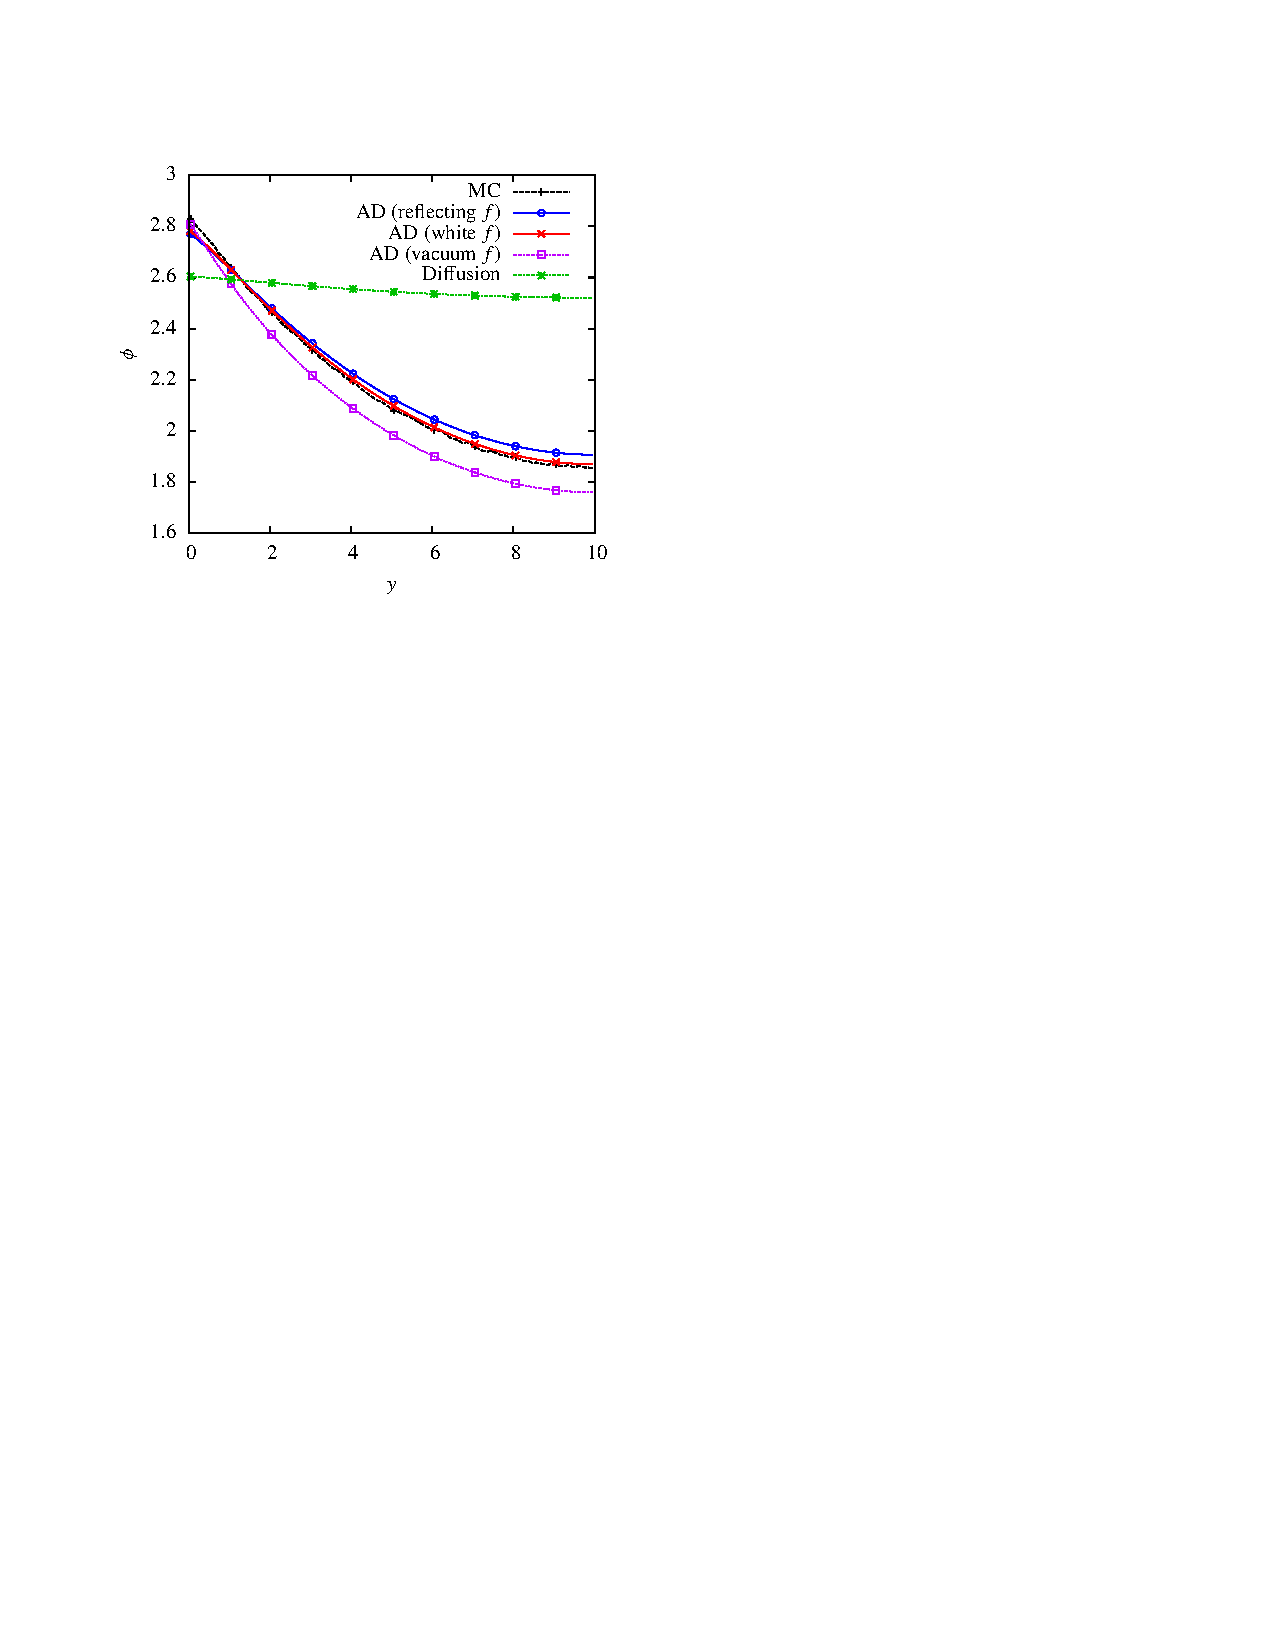
\includegraphics{example_figure}
  \caption{Captions are flush with the left.}
  \label{fig:voltage}
\end{figure}

Later on, we can include a table, even one that spans two columns such as
Table~\ref{tab:widetable}.
%%%%%%%%%%%%%%%%%%%%%%%%%%%%%%%%%%%%%%%%
\begin{table*}[htb]
  \centering
\begin{tabular}{llllllllll}\toprule
      & $\phi_T(0)$      & $\phi_T(10)$      & $\phi_T(20)$      &
      $\phi_D(0)$      & $\phi_D(10)$      & $\phi_D(20)$      & $\rho$      &
      $\varepsilon$      & $N_\text{it}$
\\ \midrule
$c=0.999$  & 0.9038 & 20.63 & 31.24 & 0.9087 & 20.63 & 31.23 & 0.2192 & $10^{-7}$ & 15
\\
$c=0.990$  & 0.3675 & 13.04 & 24.7 & 0.3696 & 13.04 & 24.69 & 0.2184 & $10^{-7}$ & 15
\\
$c=0.900$  & 0.009909 & 4.776 & 17.64 & 0.009984 & 4.786 & 17.63 & 0.2118 & $10^{-7}$ & 14
\\
$c=0.500$  & $6.069\times 10^{-5}$ & 2.212 & 15.53 & 6.213$\times 10^{-5}$ & 2.239 & 15.53 & 0.2068 & $10^{-7}$ & 13
\\
\bottomrule
\end{tabular}
  \caption{This is an example of a really wide table which might not normally
  fit in the document.}
  \label{tab:widetable}
\end{table*}
%%%%%%%%%%%%%%%%%%%%%%%%%%%%%%%%%%%%%%%%
Notice how the table reference uses a Roman numeral
for its numbering scheme, whereas the figure reference uses an Arabic numeral.
For one-column tables, use the \verb|table| environment; two-column tables use
\verb|table*|. The same applies to figures.

%%%%%%%%%%%%%%%%%%%%%%%%%%%%%%%%%%%%%%%%%%%%%%%%%%%%%%%%%%%%%%%%%%%%%%%%%%%%%%%%
\subsection{Another Subsection}
Excessive sectioning in a three-page document is discouraged, but here are more
subsections to demonstrate compliance with the ANS formatting guidelines.

\subsubsection{Third-level Heading}
This subsubsection shows compliance with the ANS-specified standard. This level
of heading should be used rarely.

\subsubsection{Another Such Heading}
And, if you really think you need a third-level heading, you should make sure
that your subsection needs at least two of them.

%%%%%%%%%%%%%%%%%%%%%%%%%%%%%%%%%%%%%%%%%%%%%%%%%%%%%%%%%%%%%%%%%%%%%%%%%%%%%%%%
\section{Conclusions}

The included ANS style file and this clear example file are a panacea for
the hours of headache that invariably results from formatting a document in
Microsoft Word.

%%%%%%%%%%%%%%%%%%%%%%%%%%%%%%%%%%%%%%%%%%%%%%%%%%%%%%%%%%%%%%%%%%%%%%%%%%%%%%%%
\appendix
\section{Appendix}

Numbering in the appendix is different:
\begin{equation} \label{eq:appendix}
  2 + 2 = 5\,.
\end{equation}
and another equation:
\begin{equation} \label{eq:appendix2}
  a + b = c\,.
\end{equation}

%%%%%%%%%%%%%%%%%%%%%%%%%%%%%%%%%%%%%%%%%%%%%%%%%%%%%%%%%%%%%%%%%%%%%%%%%%%%%%%%
\section{Acknowledgments}
This material is based upon work supported a Department of Energy Nuclear
Energy University Programs Graduate Fellowship.

%%%%%%%%%%%%%%%%%%%%%%%%%%%%%%%%%%%%%%%%%%%%%%%%%%%%%%%%%%%%%%%%%%%%%%%%%%%%%%%%
\bibliographystyle{ans}
\bibliography{bibliography}
\end{document}

